
%(BEGIN_QUESTION)
% Copyright 2007, Tony R. Kuphaldt, released under the Creative Commons Attribution License (v 1.0)
% This means you may do almost anything with this work of mine, so long as you give me proper credit

Determine a basic 5-point (0\%, 25\%, 50\%, 75\%, and 100\%) calibration table for the displacer level transmitter in this scenario:

$$\includegraphics[width=15.5cm]{i02958x01.eps}$$

The cylindrical displacer weighs 10 pounds (dry) and has a diameter of 2 inches.  The process liquid is water (density = 62.428 lb/ft$^{3}$).  The 0\% process liquid level (LRV) begins when the displacer is submerged 5 inches.  Assume a pneumatic transmitter mechanism with an output range of 3 to 15 PSI, and a calibration tolerance of $\pm$ 1\% (of span).

% No blank lines allowed between lines of an \halign structure!
% I use comments (%) instead, so that TeX doesn't choke.

$$\vbox{\offinterlineskip
\halign{\strut
\vrule \quad\hfil # \ \hfil & 
\vrule \quad\hfil # \ \hfil & 
\vrule \quad\hfil # \ \hfil & 
\vrule \quad\hfil # \ \hfil & 
\vrule \quad\hfil # \ \hfil \vrule \cr
\noalign{\hrule}
%
% First row
Percent of & Buoyant & Output signal & Output signal & Output signal \cr
%
% Another row
span (\%) & force (lb) & ideal (PSI) & min. (PSI) & max. (PSI) \cr
%
\noalign{\hrule}
%
% Another row
0 &  &  &  &  \cr
%
\noalign{\hrule}
%
% Another row
25 &  &  &  &  \cr
%
\noalign{\hrule}
%
% Another row
50 &  &  &  &  \cr
%
\noalign{\hrule}
%
% Another row
75 &  &  &  &  \cr
%
\noalign{\hrule}
%
% Another row
100 &  &  &  &  \cr
%
\noalign{\hrule}
} % End of \halign 
}$$ % End of \vbox

\vskip 10pt

Be sure to show all your mathematical work so that your instructor will be able to check the conceptual validity of your technique(s).  A good way to check to see if you're solving the problem correctly is to check that each and every one of your intermediate calculations (i.e. the results you get mid-way during the process to arrive at the final answer) has real physical meaning.  {\bf If you truly understand what you are doing, you will be able to identify the correct unit of measurement for every intermediate result and also be able to show where that number applies to the scenario at hand}.


\vskip 20pt \vbox{\hrule \hbox{\strut \vrule{} {\bf Suggestions for Socratic discussion} \vrule} \hrule}

\begin{itemize}
\item{} What effect would accidently leaving the lower block valve closed have on this instrument upon process start-up?
\item{} What effect would accidently leaving the upper block valve closed have on this instrument upon process start-up?
\item{} Describe a complete {\it wet} calibration procedure for this level transmitter.
\item{} Describe a complete {\it dry} calibration procedure for this level transmitter.
\item{} Demonstrate how to {\it estimate} numerical answers for this problem without using a calculator.
\end{itemize}

\underbar{file i02958}
%(END_QUESTION)





%(BEGIN_ANSWER)

\noindent
{\bf Partial answer:}

\vskip 10pt

% No blank lines allowed between lines of an \halign structure!
% I use comments (%) instead, so that TeX doesn't choke.

$$\vbox{\offinterlineskip
\halign{\strut
\vrule \quad\hfil # \ \hfil & 
\vrule \quad\hfil # \ \hfil & 
\vrule \quad\hfil # \ \hfil & 
\vrule \quad\hfil # \ \hfil & 
\vrule \quad\hfil # \ \hfil \vrule \cr
\noalign{\hrule}
%
% First row
Percent of & Buoyant & Output signal & Output signal & Output signal \cr
%
% Another row
span (\%) & force (lb) & ideal (PSI) & min. (PSI) & max. (PSI) \cr
%
\noalign{\hrule}
%
% Another row
0 & 0.5675 & 3 &  &  \cr
%
\noalign{\hrule}
%
% Another row
25 &  &  & 5.88 &  \cr
%
\noalign{\hrule}
%
% Another row
50 & 1.929 &  & 8.88 &  \cr
%
\noalign{\hrule}
%
% Another row
75 &  &  &  & 12.12 \cr
%
\noalign{\hrule}
%
% Another row
100 & 3.291 & &  & 15.12 \cr
%
\noalign{\hrule}
} % End of \halign 
}$$ % End of \vbox


%(END_ANSWER)





%(BEGIN_NOTES)

Total displacer volume = (29 in)($\pi$) = 91.11 in$^{3}$ = 0.05272 ft$^{3}$

$$F_{buoyant} = \gamma V$$

URV buoyancy = (62.428 lb/ft$^{3}$)(0.05272 ft$^{3}$) = 3.291 lb

LRV buoyancy = 5/29 URV buoyancy = 0.5675 lb

% No blank lines allowed between lines of an \halign structure!
% I use comments (%) instead, so that TeX doesn't choke.

$$\vbox{\offinterlineskip
\halign{\strut
\vrule \quad\hfil # \ \hfil & 
\vrule \quad\hfil # \ \hfil & 
\vrule \quad\hfil # \ \hfil & 
\vrule \quad\hfil # \ \hfil & 
\vrule \quad\hfil # \ \hfil \vrule \cr
\noalign{\hrule}
%
% First row
Percent of & Buoyant & Output signal & Output signal & Output signal \cr
%
% Another row
span (\%) & force (lb) & ideal (PSI) & min. (PSI) & max. (PSI) \cr
%
\noalign{\hrule}
%
% Another row
0 & 0.5675 & 3 & 2.88 & 3.12 \cr
%
\noalign{\hrule}
%
% Another row
25 & 1.248 & 6 & 5.88 & 6.12 \cr
%
\noalign{\hrule}
%
% Another row
50 & 1.929 & 9 & 8.88 & 9.12 \cr
%
\noalign{\hrule}
%
% Another row
75 & 2.610 & 12 & 11.88 & 12.12 \cr
%
\noalign{\hrule}
%
% Another row
100 & 3.291 & 15 & 14.88 & 15.12 \cr
%
\noalign{\hrule}
} % End of \halign 
}$$ % End of \vbox

\vskip 10pt

The 350 PSI vapor pressure is extraneous information, included for the purpose of challenging students to identify whether or not information is relevant to solving a particular problem.

















\vfil \eject

\noindent
{\bf Summary Quiz:}

Suppose a cylindrical displacer 3.5 inches in diameter hangs vertically, 2 feet of its length submerged in a liquid having a specific gravity of 0.88.  Calculate the amount of buoyant force this displacer experiences.

\begin{itemize}
\item{} 9.48 pounds
\vskip 5pt 
\item{} 8.34 pounds
\vskip 5pt 
\item{} 7.34 pounds
\vskip 5pt 
\item{} 1.60 pounds
\vskip 5pt 
\item{} 29.35 pounds
\vskip 5pt 
\item{} 2.34 pounds
\end{itemize}


%INDEX% Calibration: table, level transmitter
%INDEX% Measurement, level: calibration table
%INDEX% Measurement, level: displacer (buoyancy)

%(END_NOTES)


